\documentclass[11pt, twoside, fleqn]{report}

% Load first to prevent errors of unknown origin.
\usepackage{tipa}
\usepackage[backend=biber, style=ieee]{biblatex}
\usepackage[labelfont=bf]{caption}
\usepackage[margin=1in]{geometry}
\usepackage[colorlinks]{hyperref}
\usepackage[version=4]{mhchem}
\usepackage[parfill, skip=1em]{parskip}
\usepackage[para]{threeparttable}
\usepackage{amssymb, booktabs, derivative, fancyhdr, float, graphicx, microtype, multirow, natex, pgfplots, physics2, siunitx, tikz}
% Must be loaded after amsmath.
\usepackage[capitalize, nameinlink]{cleveref}
% Must be loaded after xcolor.
\usepackage{pagecolor}

% biblatex
\addbibresource{gedisabres.bib}

% fancyhdr
\setlength{\headheight}{14pt}
\renewcommand{\chaptermark}[1]{\markboth{\thechapter\ #1}{}}
\renewcommand{\sectionmark}[1]{\markright{\thesection\ #1}}
\fancypagestyle{mystyle}{
    \fancyfoot{}
    \fancyfoot[C]{\thepage}
}

% hyperref
\hypersetup{
    linkcolor = pink,
    urlcolor = green,
    citecolor = blue
}

% pagecolor
% [Catppuccin palette](https://catppuccin.com/palette/).
\definecolor{rosewater}{HTML}{f5e0dc}
\definecolor{flamingo}{HTML}{f2cdcd}
\definecolor{pink}{HTML}{f5c2e7}
\definecolor{mauve}{HTML}{cba6f7}
\definecolor{red}{HTML}{f38ba8}
\definecolor{maroon}{HTML}{eba0ac}
\definecolor{peach}{HTML}{fab387}
\definecolor{yellow}{HTML}{f9e2af}
\definecolor{green}{HTML}{a6e3a1}
\definecolor{teal}{HTML}{94e2d5}
\definecolor{sky}{HTML}{89dceb}
\definecolor{sapphire}{HTML}{74c7ec}
\definecolor{blue}{HTML}{89b4fa}
\definecolor{lavender}{HTML}{b4befe}
\definecolor{text}{HTML}{cdd6f4}
\definecolor{subtext-1}{HTML}{bac2de}
\definecolor{subtext-0}{HTML}{a6adc8}
\definecolor{overlay-2}{HTML}{9399b2}
\definecolor{overlay-1}{HTML}{7f849c}
\definecolor{overlay-0}{HTML}{6c7086}
\definecolor{surface-2}{HTML}{585b70}
\definecolor{surface-1}{HTML}{45475a}
\definecolor{surface-0}{HTML}{313244}
\definecolor{base}{HTML}{1e1e2e}
\definecolor{mantle}{HTML}{181825}
\definecolor{crust}{HTML}{11111b}
\pagecolor{base}
\color{text}

% pgfplots
\pgfplotsset{compat=newest}

% physics2
\usephysicsmodule{ab}

% siunitx
\DeclareSIUnit{\angstrom}{\text{Å}}

% custom
\newcommand{\dash}{\!-\!}
\newcommand{\state}[2]{\prescript{#1}{}{#2}}

\begin{document}

\pagestyle{empty}

\begin{titlepage}

    \raggedleft

    \rule{1pt}{\textheight}
    \hspace{0.05\textwidth}
    \parbox[b]{0.75\textwidth}{

        {\Huge\textsc{GEDISABRES}}\\
        \textipa{/"dZEdaI "seIb\textrhookschwa z/}\\[2\baselineskip]
        {\large\textit{\textcolor{red}{Ge}neralized \textcolor{peach}{Di}atomic \textcolor{yellow}{S}imulation for \textcolor{green}{Ab}sorption and \textcolor{sky}{R}ovibronic \\ \textcolor{blue}{E}mission \textcolor{lavender}{S}pectra}}\\[4\baselineskip]
        {\large Nathan G. Phillips}

        \vspace{0.5\textheight}

        {\noindent Texas A\&M University}\\[\baselineskip]
    }

\end{titlepage}

\tableofcontents
\newpage
\listoffigures
\newpage
\listoftables
\newpage

\pagestyle{mystyle}

\chapter{Quantum Numbers}
\label{c:quantum_numbers}

\section{Atoms}
\label{s:atoms}

\subsection{Atomic Term Symbol}

\begin{equation*}
    \state{2S + 1}{L_J}
\end{equation*}

\section{Molecules}
\label{s:molecules}

\subsection{Molecular Term Symbol}

\begin{equation*}
    \state{2S + 1}{\Lambda_{\Omega, (g/u)}^{(+/-)}}
\end{equation*}


\chapter{Hund's Coupling Cases}
\label{c:hunds_coupling_cases}

\section{Hund's Case (a)}
\label{s:hunds_case_a}

\subsection{Good Quantum Numbers}

\begin{equation*}
    \Lambda, S, \Sigma, J, \Omega
\end{equation*}

\subsection{Selection Rules}

General rules
\begin{align*}
    g &\nleftrightarrow g, \quad g \leftrightarrow u, \quad u \nleftrightarrow u \\
    \adif{J} &= 0, \pm 1 \text{ with the restriction } J = 0 \nrightarrow J = 0
\end{align*}

Rules common to both (a) and (b)
\begin{align*}
    \adif{\Lambda} &= 0, \pm 1 \\
    \adif{S} &= 0
\end{align*}

Rules for case (a) only
\begin{align*}
    \adif{\Sigma} &= 0 \\
    \adif{\Omega} &= 0, \pm 1 \\
    \adif{J} &= 0 \text{ is forbidden for } \Omega = 0 \rightarrow \Omega = 0
\end{align*}

\subsection{Term Values}

\begin{equation*}
    F_v(J) = B_v[J(J + 1) - \Omega^2]
\end{equation*}

\section{Hund's Case (b)}
\label{s:hunds_case_b}

\subsection{Good Quantum Numbers}

\begin{equation*}
    \Lambda, N, S, J
\end{equation*}

\subsection{Selection Rules}

General rules
\begin{align*}
    g &\nleftrightarrow g, \quad g \leftrightarrow u, \quad u \nleftrightarrow u \\
    \adif{J} &= 0, \pm 1 \text{ with the restriction } J = 0 \nrightarrow J = 0
\end{align*}

Rules common to both (a) and (b)
\begin{align*}
    \adif{\Lambda} &= 0, \pm 1 \\
    \adif{S} &= 0
\end{align*}

Rules for case (b) only
\begin{align*}
    \adif{N} &= 0, \pm 1 \\
    \adif{N} &= 0 \text{ is forbidden for } \Sigma\dash\Sigma \text{ transitions}
\end{align*}

\subsection{Term Values}

$\state{2}{\Sigma}$ states
\begin{align*}
    F_1(N) &= B_vN(N + 1) + \tfrac{1}{2}\gamma N \\
    F_2(N) &= B_vN(N + 1) - \tfrac{1}{2}\gamma(N + 1)
\end{align*}

$\state{3}{\Sigma}$ states
\begin{align*}
    F_1(N) &= B_vN(N + 1) + (2N + 3)B_v - \lambda - \sqrt{(2N + 3)^2B_v^2 + \lambda^2 - 2\lambda B_v} + \gamma(N + 1) \\
    F_2(N) &= B_vN(N + 1) \\
    F_3(N) &= B_vN(N + 1) - (2N - 1)B_v - \lambda + \sqrt{(2N - 1)^2B_v^2 + \lambda^2 - 2\lambda B_v} - \gamma N
\end{align*}


\chapter{Energy}

\section{Total Energy}

According to the Born--Oppenheimer approximation, the total energy of a molecule can be approximated as the sum of electronic, vibrational, and rotational components; that is \cite[149]{herzbergMolecularSpectraMolecular1950}
\begin{equation*}
    E = E_e + E_v + E_r.
\end{equation*}
In molecular spectroscopy, the components of interest are the electronic, vibrational, and rotational energies. Writing this equation using term values yields
\begin{equation*}
    T = T_e + G + F.
\end{equation*}
The wave numbers of the spectral lines corresponding to the transitions between two electronic states are given by
\begin{equation*}
    \nu = T' - T'' = (T_e' - T_e'') + (G' - G'') + (F' - F'').
\end{equation*}
This equation implies that the emitted or absorbed frequencies are composed of the electronic, vibrational, and rotational components:
\begin{equation*}
    \nu = \nu_e + \nu_v + \nu_r.
\end{equation*}

\section{Rotational Structure}

For a vibronic transition, the quantity
\begin{equation*}
    \nu_0 = \nu_e + \nu_v,
\end{equation*}
called the band origin, is constant, while $\nu_r$ is variable and depends on the value of the rotational quantum numbers of the upper and lower states \cite[168]{herzbergMolecularSpectraMolecular1950}. Therefore, the wavenumbers of a rovibrational band can be computed as
\begin{equation*}
    \nu = \nu_0 + F'(J') - F''(J'').
\end{equation*}

\section{Term Values}

The term values of the vibrating rotator can be expressed in the form of a double power series called the Dunham expansion, where \cite[109]{herzbergMolecularSpectraMolecular1950}
\begin{equation*}
    T = \sum_{lj}Y_{lj}\ab(v + \tfrac{1}{2})^l [J(J + 1)]^j.
\end{equation*}
The relations between Dunham coefficients $Y_{lj}$ and spectroscopic constants are shown below in \cref{t:dunham_coefficients}.
\begin{table}[H]
    \centering
    \caption{Relations between Dunham coefficients and spectroscopic constants \cite[419]{babouHighTemperatureNonequilibriumPartition2009}.}
    \label{t:dunham_coefficients}
    \begin{tabular}{c|ccccc}
        \toprule
        $l$ & $j = 0$            & $j = 1$           & $j = 2$      & $j = 3$ & $j = 4$ \\
        \midrule
        0   & $Y_{00}$           & $B_e$           & $-D_e$     & $H_e$ & $L_e$ \\
        1   & $\omega_e$       & $-\alpha_e$     & $-\beta_e$ &         &         \\
        2   & $-\omega_ex_e$ & $\gamma_e$      & $-g_e$     &         &         \\
        3   & $\omega_ey_e$  & $\delta_e$      & $-h_e$     &         &         \\
        4   & $\omega_ez_e$  & $\varepsilon_e$ & $-k_e$     &         &         \\
        5   & $\omega_ea_e$  & $\xi_e$         &              &         &         \\
        6   & $\omega_eb_e$  & $\eta_e$        &              &         &         \\
        7   & $\omega_ec_e$  & $\theta_e$      &              &         &         \\
        8   & $\omega_ed_e$  &                   &              &         &         \\
        9   & $\omega_ee_e$  &                   &              &         &         \\
        \bottomrule
    \end{tabular}
\end{table}
The first coefficient represents the addition to the zero-point energy above that of the anharmonic oscillator, which is \cite[109]{herzbergMolecularSpectraMolecular1950}
\begin{equation*}
    Y_{00} = \frac{B_e}{4} + \frac{\alpha_e\omega_e}{12B_e} + \frac{\alpha_e^2\omega_e^2}{144B_e^3} - \frac{\omega_ex_e}{4}.
\end{equation*}

The vibrational term value can be expanded as a power series following the approach of Dunham, which yields \cite[419]{babouHighTemperatureNonequilibriumPartition2009}
\begin{align*}
    G & = \omega_e\ab(v + \tfrac{1}{2}) - \omega_ex_e\ab(v + \tfrac{1}{2})^2 + \omega_ey_e\ab(v + \tfrac{1}{2})^3 + \omega_ez_e\ab(v + \tfrac{1}{2})^4 + \omega_ea_e\ab(v + \tfrac{1}{2})^5 \\
    & + \omega_eb_e\ab(v + \tfrac{1}{2})^6 + \omega_ec_e\ab(v + \tfrac{1}{2})^7 + \omega_ed_e\ab(v + \tfrac{1}{2})^8 + \omega_ee_e\ab(v + \tfrac{1}{2})^9 + \dotsb.
\end{align*}
Similarly, expansion of the rotational term value gives
\begin{equation*}
    F = B_vJ(J + 1) - D_v[J(J + 1)]^2 + H_v[J(J + 1)]^3 + L_v[J(J + 1)]^4 + \dotsb.
\end{equation*}
Note that the rotational expansion in particular is only a rough approximation and does not include the fine structure effects caused by spin-spin, spin-orbit, or spin-rotation coupling.
These additions are made depending on the specific molecule under consideration.
The rotational constants present within the rotational term value are expressed as
\begin{align*}
    B_v & = B_e - \alpha_e\ab(v + \tfrac{1}{2}) + \gamma_e\ab(v + \tfrac{1}{2})^2 + \delta_e\ab(v + \tfrac{1}{2})^3 + \varepsilon_e\ab(v + \tfrac{1}{2})^4 + \xi_e\ab(v + \tfrac{1}{2})^5 + \eta_e\ab(v + \tfrac{1}{2})^6 \\
    & + \theta_e\ab(v + \tfrac{1}{2})^7 + \dotsb,                                                                                                                                                                                         \\
    D_v & = D_e + \beta_e\ab(v + \tfrac{1}{2}) + g_e\ab(v + \tfrac{1}{2})^2 + h_e\ab(v + \tfrac{1}{2})^3 + k_e\ab(v + \tfrac{1}{2})^4 + \dotsb,                                                                                   \\
    H_v & = H_e + \dotsb,
\end{align*}
and
\begin{equation*}
    L_v = L_e + \dotsb.
\end{equation*}

The Hamiltonian for the $X\state{3}{\Sigma}_g^{-}$ ground state of \ce{O2} can be expressed as the sum of rotational, spin-spin, and spin-rotation interactions.
Namely, \cite[1394]{amiotMagneticDipole1Dg1981}
\begin{equation*}
    H = H_r + H_{ss} + H_{sr},
\end{equation*}
where
\begin{align*}
    H_r  & = B\vb{N}^2 - D\vb{N}^4,                    \\
    H_{ss} & = \tfrac{2}{3}\lambda(3S_z^2 - \vb{S}^2),
\end{align*}
and
\begin{equation*}
    H_{sr} = \gamma\vb{N}\vdot\vb{S}.
\end{equation*}
The spin-spin and spin-rotation coupling constants, $\lambda$ and $\gamma$ respectively, can be written as
\begin{align*}
    \lambda & = \lambda_0 + \lambda_1\vb{N}^2 \\
    \gamma  & = \gamma_0 + \gamma_1\vb{N}^2.
\end{align*}

In a Hund's case (b) basis, the matrix representation of the three Hamiltonians for a given $J$ is \cite[1394]{amiotMagneticDipole1Dg1981}
\begin{align*}
    H_r                                          & = B\bmx{
        J(J - 1)                                       & 0                                                        & 0                   \\
        0                                              & (J + 1)(J + 2)                                           & 0                   \\
        0                                              & 0                                                        & J(J + 1)
    }                                                                                                                               \\
    & - D\bmx{
        J^2(J - 1)^2                               & 0                                                        & 0                   \\
        0                                              & (J + 1)^2(J + 2)^2                                   & 0                   \\
        0                                              & 0                                                        & J^2(J + 1)^2
    }                                                                                                                               \\
    H_{ss}                                         & = \lambda_0\bmx{
        \frac{2}{3} - \frac{2J}{2J + 1}                & \frac{2\sqrt{J(J + 1)}}{2J + 1}                          & 0                   \\
        \frac{2\sqrt{J(J + 1)}}{2J + 1}                & \frac{2}{3} - \frac{2(J + 1)}{2J + 1}                    & 0                   \\
        0                                              & 0                                                        & \frac{2}{3}
    }                                                                                                                               \\
    & + \lambda_1\bmx{
        \ab(\frac{2}{3} - \frac{2J}{2J + 1})J(J - 1)   & \frac{2\sqrt{J(J + 1)}}{2J + 1}(J^2 + J + 1)           & 0                   \\
        \frac{2\sqrt{J(J + 1)}}{2J + 1}(J^2 + J + 1) & \ab(\frac{2}{3} - \frac{2(J + 1)}{2J + 1})(J + 1)(J + 2) & 0                   \\
        0                                              & 0                                                        & \frac{2}{3}J(J + 1)
    }                                                                                                                               \\
    H_{sr}                                         & = \gamma_0\bmx{
        J - 1                                          & 0                                                        & 0                   \\
        0                                              & -(J + 2)                                                 & 0                   \\
        0                                              & 0                                                        & -1
    }
    + \gamma_1\bmx{
        J(J - 1)^2                                   & 0                                                        & 0                   \\
        0                                              & -(J + 2)^2(J + 1)                                      & 0                   \\
        0                                              & 0                                                        & -J(J + 1)
    }.
\end{align*}

Using the same Hamiltonian, the combined matrix elements in a Hund's case (a) basis can also be written as \cite[3]{cheungMolecularSpectroscopicConstants1986}
\begin{align*}
    F_2      & = T + Bx - Dx^2 + \tfrac{2}{3}\lambda - \gamma + \tfrac{2}{3}\lambda_Dx - \gamma_Dx, \\
    F_1F_3 & = \bmx{
        H_{11}     & H_{12}                                                                                     \\ H_{21} & H_{22}
    },
\end{align*}
where
\begin{align*}
    H_{11} & = T + B(x + 2) - D(x^2 + 8x + 4) - \tfrac{4}{3}\lambda - 2\gamma - \tfrac{4}{3}\lambda_D(x + 2) - 4\gamma_D(x + 1) \\
    H_{12} & = -2\sqrt{x}\ab[B - 2D(x + 1) - \tfrac{\gamma}{2} - \tfrac{2}{3}\lambda_D - \tfrac{1}{2}\gamma_D(x + 4)]             \\
    H_{21} & = H_{12}                                                                                                                 \\
    H_{22} & = T + Bx - D(x^2 + 4x) + \tfrac{2}{3}\lambda - \gamma + \tfrac{2}{3}x\lambda_D - 3x\gamma_D.
\end{align*}
Note that
\begin{equation*}
    x = J(J + 1).
\end{equation*}

\section{Main and Satellite Branches}

The six main branches in $\state{3}{\Sigma}\dash\state{3}{\Sigma}$ transitions are \cite[249]{herzbergMolecularSpectraMolecular1950}
\begin{align*}
    P_1 & = \nu_0 + F'_1(J - 1) - F''_1(J)  \\
    R_1 & = \nu_0 + F'_1(J + 1) - F''_1(J)  \\
    P_2 & = \nu_0 + F'_2(J - 1) - F''_2(J)  \\
    R_2 & = \nu_0 + F'_2(J + 1) - F''_2(J)  \\
    P_3 & = \nu_0 + F'_3(J - 1) - F''_3(J)  \\
    R_3 & = \nu_0 + F'_3(J + 1) - F''_3(J).
\end{align*}
The six satellite branches are
\begin{align*}
    \state{P}{Q}_{12} & = \nu_0 + F'_1(J - 1) - F''_2(J)  \\
    \state{R}{Q}_{21} & = \nu_0 + F'_2(J + 1) - F''_1(J)  \\
    \state{P}{Q}_{13} & = \nu_0 + F'_1(J - 1) - F''_3(J)  \\
    \state{R}{Q}_{31} & = \nu_0 + F'_3(J + 1) - F''_1(J)  \\
    \state{P}{Q}_{23} & = \nu_0 + F'_2(J - 1) - F''_3(J)  \\
    \state{R}{Q}_{32} & = \nu_0 + F'_3(J + 1) - F''_2(J).
\end{align*}


\chapter{Hamiltonians}

\begin{table}[H]
    \centering
    \caption{Inherent angular momenta and their quantum numbers \cite[72]{lefebvre-brionSpectraDynamicsDiatomic2004}.}
    \begin{threeparttable}
        \begin{tabular}{lcccc}
            \toprule
            \multirow{2}{*}{\textbf{Type}}          & \multicolumn{2}{c}{\textbf{Total}} & \multicolumn{2}{c}{\textbf{Projection onto INA}\tnote{\dag}}                                                    \\
            \cmidrule(lr){2-3} \cmidrule(lr){4-5}
            & \textbf{Operator}                  & \textbf{QN}\tnote{\ddag}                             & \textbf{Operator} & \textbf{QN}                  \\
            \midrule
            Nuclear spin of A                       & $\vop{I}_A$                        & $I_A$                                   & $\sop{I}_{Az}$    & no standard                  \\
            Nuclear spin of B                       & $\vop{I}_B$                        & $I_B$                                   & $\sop{I}_{Bz}$    & no standard                  \\
            Orbital ang. mom. of the $i$th electron & $\vop{l}_i$                        & $l_i$                                   & $\sop{l}_{iz}$    & $\lambda_i = 0, 1, 2, \dots$ \\
            Spin of the $i$th electron              & $\vop{s}_i$                        & $s_i$                                   & $\sop{s}_{iz}$    & $\sigma_i = \pm\frac{1}{2}$  \\
            Rotational ang. mom.                    & $\vop{R}$                          & $R$                                     & $\sop{R}_z$       & zero                         \\
            \bottomrule
        \end{tabular}
        \begin{tablenotes}
        \item [\dag] internuclear axis
        \item [\ddag] quantum number
        \end{tablenotes}
    \end{threeparttable}
\end{table}

\begin{table}[H]
    \centering
    \caption{Coupled angular momenta and their quantum numbers \cite[72]{lefebvre-brionSpectraDynamicsDiatomic2004}.}
    \begin{tabular}{lcccc}
        \toprule
        \multirow{2}{*}{\textbf{Type}}        & \multicolumn{2}{c}{\textbf{Total}}                & \multicolumn{2}{c}{\textbf{Projection onto INA}}                                                         \\
        \cmidrule(lr){2-3} \cmidrule(lr){4-5}
        & \textbf{Operator}                                 & \textbf{QN}                             & \textbf{Operator} & \textbf{QN}                       \\
        \midrule
        Total nuclear spin                    & $\vop{I} = \vop{I}_A + \vop{I}_B$                 & $I$                                     & $\sop{I}_z$       & no standard                       \\
        Total ang. mom. of the $i$th electron & $\vop{j}_i = \vop{l}_i + \vop{s}_i$               & $j_i$                                   & $\sop{j}_i$       & $\omega_i = \lambda_i + \sigma_i$ \\
        Total electron orbital ang. mom.      & $\vop{L} = \sum_i\vop{l}_i$                       & $L$                                     & $\sop{L}_z$       & $\Lambda = 0, 1, 2, \dots$        \\
        Total electron spin ang. mom.         & $\vop{S} = \sum_s\vop{s}_i$                       & $S$                                     & $\sop{S}_z$       & $\Sigma$                          \\
        Total ang. mom. w/o any spin          & $\vop{N} = \vop{R} + \vop{L}$                     & $N$                                     & $\sop{N}_z$       & $\Lambda$                         \\
        Total ang. mom. w/o nuclear spin      & $\vop{J} = \vop{R} + \vop{L} + \vop{S}$           & $J$                                     & $\sop{J}_z$       & $\Omega = \Lambda + \Sigma$       \\
        Total ang. mom.                       & $\vop{F} = \vop{R} + \vop{L} + \vop{S} + \vop{I}$ & $F$                                     & $\sop{F}_z$       & no standard                       \\
        \bottomrule
    \end{tabular}
\end{table}

\begin{table}[H]
    \centering
    \caption{Hund's coupling cases and their respective descriptions \cite[2]{hougenCalculationRotationalEnergy1970} and \cite[103]{lefebvre-brionSpectraDynamicsDiatomic2004}.}
    \begin{tabular}{cccc}
        \toprule
        \textbf{Hund's Case} & \textbf{Rotational Energy} & \textbf{Good Quantum Numbers}                 & \textbf{Degeneracy}     \\
        \midrule
        (a)                  & $BJ(J + 1)$                & $\ket{JS\Omega\Lambda\Sigma}$                 & 2 or 1                  \\
        (b)                  & $BN(N + 1)$                & $\ket{JNS\Lambda(S_R)}$                       & $2(2S + 1)$ or $2S + 1$ \\
        (c)                  & $BJ(J + 1)$                & $\ket{J[J_a]\Omega}$                          & 2 or 1                  \\
        (d)                  & $BR(R + 1)$                & $\ket{JNS(S_R)J_+N_+S_+\Lambda_+l(l_R, s_R)}$ & $(2L + 1)(2S + 1)$      \\
        \bottomrule
    \end{tabular}
\end{table}

\begin{table}[H]
    \centering
    \renewcommand{\arraystretch}{1.5}
    \caption{First-order terms in the diatomic Hamiltonian \cite[232-233]{westernPGOPHERProgramSimulating2017}.}
    \begin{tabular}{lll}
        \toprule
        \textbf{Operator} & \textbf{Equation}                                                                                         & \textbf{Condition}      \\
        \midrule
        Rotation          & $B\vop{N}^2$                                                                                              & always                  \\
        \cmidrule{2-3}
        \multirow{2}{*}{Spin-Rotation}
        & $\gamma\ab(\vop{N}\vdot\vop{S})$                                                                          & $S > 0$                 \\
        & $-\sqrt{70/3}\gamma_ST_0^2\acomm*{T^1(\vop{J})}{T^3(\vop{S})}$                                            & $S > 1$                 \\
        \cmidrule{2-3}
        \multirow{2}{*}{Spin-Orbit}
        & $A\ab(\vop{L}\vdot\vop{S})$                                                                               & $\Lambda > 0$, $S > 0$  \\
        & $\eta\sop{L}_z\sop{S}_z\ab[\sop{S}_z^2 - \frac{1}{5}\ab(3\vop{S}^2 - 1)]$                                 & $\Lambda > 0$, $S > 1$  \\
        \cmidrule{2-3}
        \multirow{2}{*}{Spin-Spin}
        & $\frac{2}{3}\lambda\ab(3\sop{S}_z^2 - \vop{S}^2)$                                                         & $S > 1/2$               \\
        & $\frac{1}{12}\theta\ab(35\sop{S}_z^4 - 30\vop{S}^2\sop{S}_z^2 + 25\sop{S}_z^2 - 6\vop{S}^2 + 3\vop{S}^4)$ & $S > 3/2$               \\
        \cmidrule{2-3}
        \multirow{3}{*}{$\Lambda$ Doubling}
        & $\frac{1}{2}q\ab(\sop{N}_+^2e^{-2i\phi} + \sop{N}_-^2e^{2i\phi})$                                         & $\Pi$ states            \\
        & $-\frac{1}{2}p\ab(\sop{N}_+\sop{S}_+e^{-2i\phi} + \sop{N}_-\sop{S}_-e^{2i\phi})$                          & $\Pi$ states, $S > 0$   \\
        & $\frac{1}{2}o\ab(\sop{S}_+^2e^{-2i\phi} + \sop{S}_-^2e^{2i\phi})$                                         & $\Pi$ states, $S > 1/2$ \\
        \bottomrule
    \end{tabular}
\end{table}


\chapter{Intensity}

\section{H\"onl--London Factors}

The rotational line strength factors for $\state{3}{\Sigma}^{\pm}\dash\state{3}{\Sigma}^{\pm}$ transitions are shown below in \cref{t:honl_london_factors_3s}.
\begin{table}[H]
    \centering
    \caption{H\"onl--London Factors for $\state{3}{\Sigma}^{\pm}\dash\state{3}{\Sigma}^{\pm}$ transitions \cite[2945]{tatumHonlLondonFactors1966}.}
    \label{t:honl_london_factors_3s}
    \begin{tabular}{ccc}
        \toprule
        Branch              & Emission                                & Absorption                                 \\
        \midrule
        $P_1$             & $\dfrac{(N' + 1)(2N' + 5)}{2N' + 3}$    & $\dfrac{N''(2N'' + 3)}{2N'' + 1}$          \\
        \addlinespace[0.5em]
        $R_1$             & $\dfrac{N'(2N' + 3)}{2N' + 1}$          & $\dfrac{(N'' + 1)(2N'' + 5)}{2N'' + 3}$    \\
        \addlinespace[0.5em]
        $\state{P}{Q}_{13}$ & $\dfrac{1}{(N' + 1)(2N' + 1)(2N' + 3)}$ & $\dfrac{1}{N''(2N'' - 1)(2N'' + 1)}$       \\
        \addlinespace[0.5em]
        $\state{P}{Q}_{12}$ & $\dfrac{1}{N' + 1}$                     & $\dfrac{1}{N''}$                           \\
        \addlinespace[0.5em]
        $P_2$             & $\dfrac{N'(N' + 2)}{N' + 1}$            & $\dfrac{(N'' - 1)(N'' + 1)}{N''}$          \\
        \addlinespace[0.5em]
        $R_2$             & $\dfrac{(N' - 1)(N' + 1)}{N'}$          & $\dfrac{N''(N'' + 2)}{N'' + 1}$            \\
        \addlinespace[0.5em]
        $\state{P}{Q}_{23}$ & $\dfrac{1}{N' + 1}$                     & $\dfrac{1}{N''}$                           \\
        \addlinespace[0.5em]
        $\state{R}{Q}_{21}$ & $\dfrac{1}{N'}$                         & $\dfrac{1}{N'' + 1}$                       \\
        \addlinespace[0.5em]
        $P_3$             & $\dfrac{(N' + 1)(2N' - 1)}{2N' + 1}$    & $\dfrac{N''(2N'' - 3)}{2N'' - 1}$          \\
        \addlinespace[0.5em]
        $R_3$             & $\dfrac{N'(2N' - 3)}{2N' - 1}$          & $\dfrac{(N'' + 1)(2N'' - 1)}{2N'' + 1}$    \\
        \addlinespace[0.5em]
        $\state{R}{Q}_{32}$ & $\dfrac{1}{N'}$                         & $\dfrac{1}{N'' + 1}$                       \\
        \addlinespace[0.5em]
        $\state{R}{Q}_{31}$ & $\dfrac{1}{N'(2N' - 1)(2N' + 1)}$       & $\dfrac{1}{(N'' + 1)(2N'' + 1)(2N'' + 3)}$ \\
        \bottomrule
    \end{tabular}
\end{table}

\section{Transition Intensities}

In terms of the spectral radiance $I_\nu$, the amount of radiant energy $\odif{E_\nu}$ transmitted across an element of area $\odif{\sigma}$ over solid angle $\odif{\Omega}$ in a wavenumber interval $\odif{\nu}$ during a time $\odif{t}$ is \cite[1]{chandrasekharRadiativeTransfer2016}
\begin{equation*}
    \odif{E_\nu} = I_\nu\cos\theta\odif{\nu}\odif{\sigma}\odif{\Omega}\odif{t},
\end{equation*}
where the units of spectral radiance are \unit{W.m^{-2}.sr^{-1}.1/cm^{-1}}.
Define the emission coefficient $j_\nu$ such that
\begin{equation*}
    \odif{I_\nu} = j_\nu\odif{s},
\end{equation*}
with units \unit{W.m^{-3}.sr^{-1}.1/cm^{-1}} \cite[9]{rybickiRadiativeProcessesAstrophysics2004}.
In terms of Einstein coefficients, this can be expressed as \cite[31]{rybickiRadiativeProcessesAstrophysics2004}
\begin{equation*}
    j_\nu = \frac{hc\nu_0}{4\pi}N_2A_{21}\phi(\nu).
\end{equation*}
Similarly, define the absorption coefficient $\alpha_\nu$ such that
\begin{equation*}
    \odif{I_\nu} = -\alpha_\nu I_\nu\odif{s},
\end{equation*}
with units \unit{m^{-1}} \cite[10]{rybickiRadiativeProcessesAstrophysics2004}.
In terms of Einstein coefficients, this can be expressed as \cite[31]{rybickiRadiativeProcessesAstrophysics2004}
\begin{equation*}
    \alpha_\nu = \frac{hc\nu_0}{4\pi}(N_1B_{12} - N_2B_{21})\phi(\nu).
\end{equation*}

\subsection{Einstein Coefficients}

The Einstein transition probability of spontaneous emission is \cite[21]{herzbergMolecularSpectraMolecular1950}
\begin{equation*}
    A_{nm} = \frac{64\pi^4\nu_{nm}^3}{3h}\frac{\sum\abs{\vb{R}_{n_im_k}}^2}{d_n}.
\end{equation*}
Similarly, the Einstein transition probability of absorption is
\begin{equation*}
    B_{mn} = \frac{8\pi^3}{3h^2c}\frac{\sum\abs{\vb{R}_{n_im_k}}^2}{d_m}.
\end{equation*}
These two equations are related by
\begin{equation*}
    B_{mn} = \frac{1}{8\pi hc\nu_{nm}^3}\frac{d_n}{d_m}A_{nm}.
\end{equation*}

\subsection{Transition Moment}

The electronic transition moment is defined as \cite[199]{herzbergMolecularSpectraMolecular1950}
\begin{equation*}
    \ev{\vb{R}} = \int \psi'\vb{\mu}\psi'' \odif{\tau}.
\end{equation*}
Using the Born--Oppenheimer approximation, the total transition moment may be written as \cite[382]{herzbergMolecularSpectraMolecular1950}
\begin{equation*}
    \vb{R} = \vb{R}_e^{nm}\vb{R}_v^{v'v''}\vb{R}_r^{J'J''}
\end{equation*}
The transition probability for absorption is approximately (assuming the dipole moment integrals can be separated via the Born--Oppenheimer \& Franck--Condon principles) \cite[382]{herzbergMolecularSpectraMolecular1950}
\begin{equation*}
    B_{evr} = \frac{8\pi^3}{3h^2c}\frac{\sum\abs{\vb{R}}^2}{g_eg_vg_r} = \frac{8\pi^3}{3h^2c}\frac{\abs{\vb{R}_e^{nm}}^2}{g_e}\frac{\abs{\vb{R}_v^{v'v''}}^2}{g_v}\frac{\sum\abs{\vb{R}_r^{J'J''}}^2}{g_r}.
\end{equation*}
The electronic-vibrational transition moment is calculated directly as \cite[9]{lauxArraysRadiativeTransition1992}
\begin{equation*}
    \ev{R_e^{v'v''}}^2 = \ab(\int \psi_{v'}(r)R_e(r)\psi_{v''}(r) \odif{r})^2.
\end{equation*}
The line strength of a rovibronic transition can be written as the product of the vibronic transition moment and the H\"onl--London factor \cite[451]{schadeeUniqueDefinitionsBand1978}
\begin{equation*}
    S^{e'v'J'}_{e''v''J''} = \ev{R_e^{v'v''}}^2S^{J'}_{J''}.
\end{equation*}
The electronic-vibrational Einstein coefficient for spontaneous emission is \cite[452]{schadeeUniqueDefinitionsBand1978}
\begin{equation*}
    A^{e'v'}_{e''v''} = \frac{64\pi^4\nu^3}{3h}\frac{(2 - \delta_{0, \Lambda' + \Lambda''})}{(2 - \delta_{0, \Lambda'})}\ev{R_e^{v'v''}}^2.
\end{equation*}
Writing the total Einstein coefficient for spontaneous emission gives
\begin{equation*}
    A_{ul} = A^{e'v'}_{e''v''}A^{J'}_{J''} = \frac{64\pi^4\nu^3}{3h}\frac{(2 - \delta_{0, \Lambda' + \Lambda''})}{(2 - \delta_{0, \Lambda'})}\ev{R_e^{v'v''}}^2\frac{S^{J'}_{J''}}{(2J' + 1)}.
\end{equation*}


\chapter{Partition Functions}

\section{Partition Functions}

\subsection{General Form}

General form of the Boltzmann population distribution \cite[8]{hansonSpectroscopyOpticalDiagnostics2016}
\begin{equation*}
    \frac{N_i}{N} = \frac{g_i}{Q}\exp\ab(-\frac{\varepsilon_i}{kT})
\end{equation*}
General form of the partition function \cite[8]{hansonSpectroscopyOpticalDiagnostics2016}
\begin{equation*}
    Q = \sum_i g_i\exp\ab(-\frac{\varepsilon_i}{kT})
\end{equation*}
The total molecular partition function can be expressed as the product of the individual translational, electronic, vibrational, rotational, and nuclear components for symmetric molecules is \cite[80]{hansonSpectroscopyOpticalDiagnostics2016}
\begin{equation*}
    Q = Q_tQ_eQ_vQ_rQ_n.
\end{equation*}

\subsection{Nuclear}

See \cite[81]{hansonSpectroscopyOpticalDiagnostics2016}
\begin{equation*}
    Q_n = \prod_{i = 1}^L (2I_n + 1)
\end{equation*}

\subsection{Rotational}
Because of the rotational symmetry of certain molecules, a symmetry parameter $\sigma$ must be added to the rotational partition function to account for the multiple molecular orientations that are indistinguishable.
See \cite[125]{herzbergMolecularSpectraMolecular1950}
\begin{equation*}
    Q_r = \frac{1}{\sigma} \sum g_r\exp\ab(-\frac{\varepsilon_r}{kT})
\end{equation*}
The degeneracy of each state is
\begin{equation*}
    g_r = 2J + 1
\end{equation*}
and the rotational energy can be expressed as the term value
\begin{equation*}
    \varepsilon_r = F(J)hc.
\end{equation*}
Therefore, the rotational partition function is
\begin{equation*}
    Q_r = \frac{1}{\sigma} \sum (2J + 1)\exp\ab(-\frac{F(J)hc}{kT}).
\end{equation*}
For sufficiently large $T$ or small $B$, the rotational partition function for a molecule in the high-temperature limit is \cite[17]{hansonSpectroscopyOpticalDiagnostics2016} and \cite[125]{herzbergMolecularSpectraMolecular1950}
\begin{equation*}
    Q_r \approx \frac{1}{\sigma} \int_0^{\infty} (2J + 1)\exp\ab(-\frac{BJ(J + 1)hc}{kT}) \odif{J} = \frac{1}{\sigma}\frac{kT}{hcB}
\end{equation*}
The Boltzmann fraction is then
\begin{equation*}
    \frac{N_J}{N} = \frac{(2J + 1)}{Q_r}\exp\ab(-\frac{F(J)hc}{kT})
\end{equation*}

\subsection{Effective Rotational}

The effective rotational partition function for symmetric molecules is \cite[80]{hansonSpectroscopyOpticalDiagnostics2016}
\begin{equation*}
    Q'_r = Q_rQ_n
\end{equation*}
Similarly, the effective rotational degeneracy is \cite[80]{hansonSpectroscopyOpticalDiagnostics2016}
\begin{equation*}
    g'_r = g_rg_n
\end{equation*}
For homonuclear diatomic molecules, the effective rotational degeneracy is \cite[84]{hansonSpectroscopyOpticalDiagnostics2016}
\begin{equation*}
    g'_r = \frac{(2J + 1)}{2}\ab[(2I + 1)^2 \pm (2I + 1)]
\end{equation*}

\subsection{Vibrational}

See \cite[123]{herzbergMolecularSpectraMolecular1950}
\begin{equation*}
    Q_v = \sum g_v\exp\ab(-\frac{\varepsilon_v}{kT})
\end{equation*}
The vibrational degeneracy of each state is
\begin{equation*}
    g_v = 1,
\end{equation*}
and the vibrational energy can be expressed as the term value
\begin{equation*}
    \varepsilon_v = G(v)hc.
\end{equation*}
Therefore, the vibrational partition function is
\begin{equation*}
    Q_v = \sum \exp\ab(-\frac{G(v)hc}{kT}).
\end{equation*}
The Boltzmann fraction is then
\begin{equation*}
    \frac{N_v}{N} = \frac{1}{Q_v}\exp\ab(-\frac{G(v)hc}{kT})
\end{equation*}
The vibrational partition function can also be written in terms of the zero-point vibrational energy as
\begin{equation*}
    Q_v = \sum \exp\ab(-\frac{[G(v) - G(0)]hc}{kT}).
\end{equation*}
The Boltzmann fraction is therefore
\begin{equation*}
    \frac{N_v}{N} = \frac{1}{Q_v}\exp\ab(-\frac{[G(v) - G(0)]hc}{kT}).
\end{equation*}

\subsection{Electronic}

See \cite[544]{andersonHypersonicHighTemperatureGas2019}
\begin{equation*}
    Q_e = \sum g_e\exp\ab(-\frac{\varepsilon}{kT})
\end{equation*}
The electronic degeneracy depends on the individual states. The electronic energy can be expressed as the term value
\begin{equation*}
    \varepsilon_e = T_ehc.
\end{equation*}
Therefore, the electronic partition function is
\begin{equation*}
    Q_e = \sum g_e\exp\ab(-\frac{T_ehc}{kT}).
\end{equation*}
The Boltzmann fraction is therefore
\begin{equation*}
    \frac{N_e}{N} = \frac{g_e}{Q_e}\exp\ab(-\frac{T_ehc}{kT}).
\end{equation*}

\subsection{Translational}

See \cite[544]{andersonHypersonicHighTemperatureGas2019}
\begin{equation*}
    Q_t = \ab(\frac{2\pi mkT}{h^2})^{3/2}V,
\end{equation*}
where $V$ is the volume of the system.


\chapter{Spectral Lineshapes}
\label{c:spectral_lineshapes}

\section{Gaussian Profile}
\label{s:gaussian_profile}

The probability density function (PDF) for the Gaussian profile is
\begin{equation*}
    G(x; x_0, \sigma) = \frac{1}{\sigma\sqrt{2\pi}}\exp\ab(-\frac{(x - x_0)^2}{2\sigma^2}),
\end{equation*}
where $x$ is the desired wavenumber, $x_0$ is the intensity at a wavenumber peak, and $\sigma$ is the broadening parameter.

\section{Lorentzian Profile}
\label{s:lorentzian_profile}

The PDF for the Lorentzian profile is
\begin{equation*}
    L(x; x_0, \gamma) = \frac{1}{\pi}\ab[\frac{\gamma}{(x - x_0)^2 + \gamma^2}],
\end{equation*}
where $\gamma$ is the broadening parameter.

\section{Voigt Profile}
\label{s:voigt_profile}

The Voigt profile is a convolution of the Gaussian and Lorentzian profiles. The PDF for the Voigt profile is
\begin{equation*}
    V(x; x_0, \sigma, \gamma) = \frac{1}{\sigma\sqrt{2\pi}}\Re[w(z)],
\end{equation*}
where
\begin{equation*}
    w(z) \defn \eul^{-z^2}\erfc(-\img z) = \eul^{-z^2}\ab(1 + 
    \frac{2\img}{\sqrt{\pi}}\int_0^z \eul^{t^2} \odif{t}),
\end{equation*}
and
\begin{equation*}
    z = \frac{(x - x_0) + \img\gamma}{\sigma\sqrt{2}}.
\end{equation*}

\begin{figure}[H]
    \centering
    \begin{tikzpicture}
        \begin{axis}[axis lines=left, legend style={fill=none, draw=none}]
            \addplot[color=p1, smooth]
            {1/(1*sqrt(2*pi))*exp(-((x-0)^2)/(2*1^2))};
            \addlegendentry{Gaussian}
            \addplot[color=p2, smooth]
            {1/pi*(1/((x-0)^2+1^2))};
            \addlegendentry{Lorentzian}
            \addplot gnuplot[color=p3, smooth, no marks]
            {VP(x,1,1)};
            \addlegendentry{Voigt}
        \end{axis}
    \end{tikzpicture}
\end{figure}


\chapter{Line Shifting Mechanisms}

\section{Doppler Shift}

For molecules that have a bulk velocity $u$ relative to a laser beam, the Doppler shift is given by \cite[142]{hansonSpectroscopyOpticalDiagnostics2016}
\begin{equation*}
    \fdif{\nu}_D = \nu_0\frac{u}{c}.
\end{equation*}

\paragraph{Unit Verification}

The units of $\fdif{\nu}_D$ using the formula given are inverse centimeters, as shown by the following:
\begin{equation*}
    \fdif{\nu}_D = \unit{cm^{-1}}\frac{\unit{m.s^{-1}}}{\unit{m.s^{-1}}} = \unit{cm^{-1}}.
\end{equation*}

\section{Collisional Shift}

Line shifts due to collisional processes can be modeled as \cite[141]{hansonSpectroscopyOpticalDiagnostics2016}
\begin{equation*}
    \fdif{\nu}_C = \alpha p\ab(\frac{T_0}{T})^\beta,
\end{equation*}
where $\alpha$ is a pressure shift coefficient in \unit{cm^{-1}.Pa^{-1}} and $\beta$ is a nondimensional temperature exponent.

\paragraph{Unit Verification}

The units of $\fdif{\nu}_C$ using the formula given are inverse centimeters, as shown by the following:
\begin{equation*}
    \fdif{\nu}_C = \unit{cm^{-1}.Pa^{-1}.Pa} = \unit{cm^{-1}}.
\end{equation*}


\chapter{Laser-Induced Fluorescence}

\section{Rate Equations}

\begin{figure}[H]
    \centering
    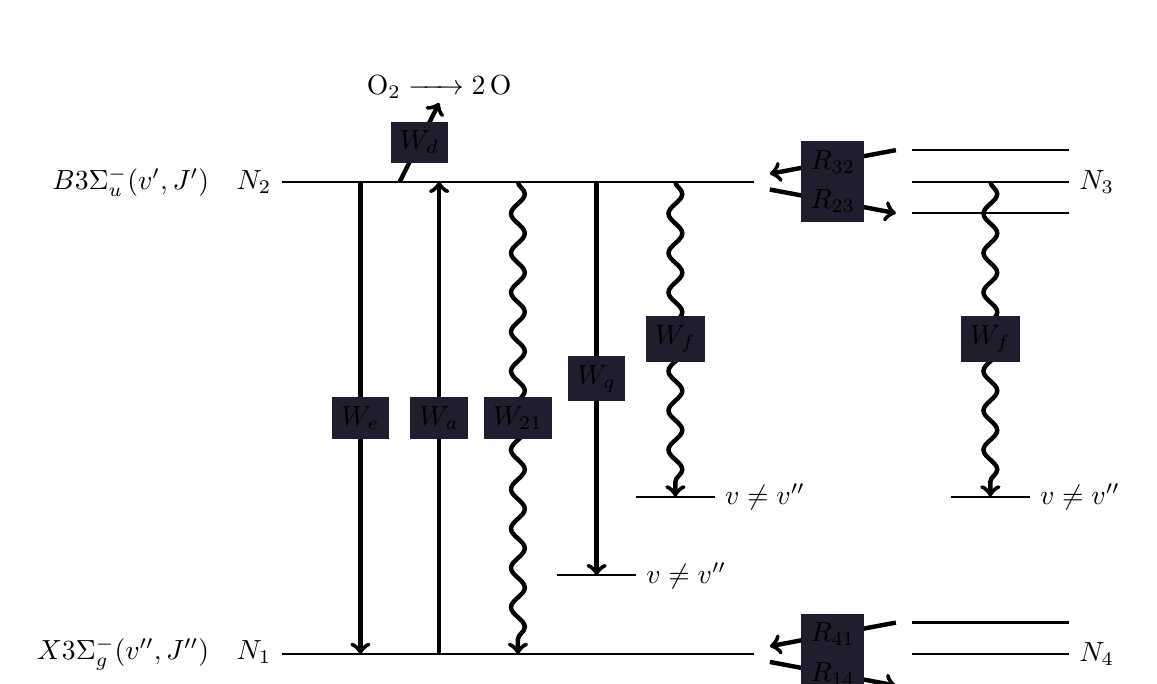
\begin{tikzpicture}
        \draw[thick] (6,0) -- (0,0) node[left] {$X\state{3}{\Sigma}_g^{-}(v'', J'') \quad N_1$};
        \draw[thick] (6,6) -- (0,6) node[left] {$B\state{3}{\Sigma}_u^{-}(v', J') \quad N_2$};

        \draw[->,ultra thick] (1,6) -- (1,0) node[midway,fill=base] {$W_e$};
        \draw[->,ultra thick] (1.5,6) -- (2,7) node[midway,fill=base] {$W_d$};
        \node at(2,7.2) {\ce{O2 -> 2O}};
        \draw[->,ultra thick] (2,0) -- (2,6) node[midway,fill=base] {$W_a$};
        \draw[->,ultra thick,decorate,decoration={snake,segment length=5mm}] (3,6) -- (3,0) node[midway,fill=base] {$W_{21}$};
        \draw[->,ultra thick] (4,6) -- (4,1) node[midway,fill=base] {$W_q$};
        \draw[thick] (3.5,1) -- (4.5,1) node[right] {$v \neq v''$};
        \draw[->,ultra thick,decorate,decoration={snake, segment length=5mm}] (5,6) -- (5,2) node[midway,fill=base] {$W_f$};
        \draw[thick] (4.5,2) -- (5.5,2) node[right] {$v \neq v''$};

        \draw[<-,ultra thick] (6.2,6.1) -- (7.8,6.4) node[midway,fill=base] {$R_{32}$};
        \draw[thick] (8,6.4) -- (10,6.4);
        \draw[thick] (8,6) -- (10,6) node[right] {$N_3$};
        \draw[thick] (8,5.6) -- (10,5.6);
        \draw[->,ultra thick] (6.2,5.9) -- (7.8,5.6) node[midway,fill=base] {$R_{23}$};

        \draw[->,ultra thick,decorate,decoration={snake,segment length=5mm}] (9,6) -- (9,2) node[midway,fill=base] {$W_f$};
        \draw[thick] (8.5,2) -- (9.5,2) node[right] {$v \neq v''$};

        \draw[<-,ultra thick] (6.2,0.1) -- (7.8,0.4) node[midway,fill=base] {$R_{41}$};
        \draw[thick] (8,0.4) -- (10,0.4);
        \draw[thick] (8,0) -- (10,0) node[right] {$N_4$};
        \draw[thick] (8,-0.4) -- (10,-0.4);
        \draw[->,ultra thick] (6.2,-0.1) -- (7.8,-0.4) node[midway,fill=base] {$R_{14}$};
    \end{tikzpicture}
    \caption{Four-level LIF model for the Schumann--Runge bands of molecular oxygen.}
\end{figure}

\subsection{Four-level LIF}

The four-level equations are \cite[18]{grinsteadTemperatureMeasurementHighTemperature1995}
\begin{align*}
    \odv{N_1}{t} & = -(W_a + R_{14})N_1 + (W_e + W_{21})N_2 + R_{41}N_4                      \\
    \odv{N_2}{t} & = W_aN_1 - (W_f + W_d + W_q + W_e + W_{21} + R_{23})N_2 + R_{32}N_3 \\
    \odv{N_3}{t} & = R_{23}N_2 - (W_f + R_{32})N_3                                               \\
    \odv{N_4}{t} & = R_{14}N_1 - R_{41}N_4
\end{align*}
$W_a$ is the laser-stimulated absorption rate, $W_e$ the laser-stimulated emission rate, $W_{21}$ the spontaneous emission rate, $W_d$ the predissociation rate, $W_q$ the collisional quenching rate, $W_f$ the fluorescent radiative decay rate, and $R_{ij}$ the rotational energy transfer rates.

\subsection{Three-level LIF}

The three-level equations are \cite[2]{diskin3LevelModelSchumann1996}
\begin{align*}
    \odv{N_1}{t} & = -W_aN_1 + (W_e + W_{21})N_2 + W_c\ab(\frac{f_b}{1 - f_b}N_3 - N_1) \\
    \odv{N_2}{t} & = W_aN_1 - (W_e + W_d + W_{21} + W_f + W_q)N_2                           \\
    \odv{N_3}{t} & = -W_c\ab(\frac{f_b}{1 - f_b}N_3 - N_1)
\end{align*}
where $f_b$ is the rotational Boltzmann fraction for the lower state.
Here, the laser rates are given by
\begin{align*}
    W_a & = I_l(t)B_{12}\phi(\nu) \\
    W_e & = I_l(t)B_{21}\phi(\nu),
\end{align*}
where $\phi(\nu)$ is the overlap integral between the transition and laser lineshapes, given as
\begin{equation*}
    \phi(\nu_t, \nu_l) = \int \phi_t(\nu)\phi_l(\nu) \odif{\nu}.
\end{equation*}
$I_l$ is the laser intensity, which can be modeled as a Gaussian distribution in time
\begin{equation*}
    I_l(t) = \frac{2\Phi}{\adif{t}}\sqrt{\frac{\ln{2}}{\pi}}\exp\ab[-4\ln{2}\ab(\frac{t - t_0}{\adif{t}})^2],
\end{equation*}
where $\Phi = E_l/A$ is the laser fluence.


\chapter{Molecular Oxygen}

\section{Selection Rules}

Conversion of $J$ to $N$ \cite[7]{grinsteadTemperatureMeasurementHighTemperature1995},
\begin{align*}
    F_1: J & = N + 1 \\
    F_2: J & = N     \\
    F_3: J & = N - 1
\end{align*}

For the three primary $P$-branch lines,
\begin{equation*}
    \adif{N} = \adif{J} = -1.
\end{equation*}
For the three primary $R$-branch lines,
\begin{equation*}
    \adif{N} = \adif{J} = +1.
\end{equation*}
For the six satellite bands,
\begin{equation*}
    \adif{N} \neq \adif{J}.
\end{equation*}
Two forbidden lines with $\adif{N} = \pm3, \adif{J} = \pm1$ have been observed.

Because of symmetry properties of the rotational levels and the influence of nuclear spin, only the rotational levels with odd $N$ can be populated in $X\state{3}{\Sigma}_g^{-}$, and only the rotational levels with even $N$ can be populated in $B\state{3}{\Sigma}_u^{-}$. See \cite[135]{herzbergMolecularSpectraMolecular1950}.

Furthermore, for $N = 0$ in $B\state{3}{\Sigma}_u^{-}$, only the $F_1$ level exists.

\begin{figure}[H]
    \centering
    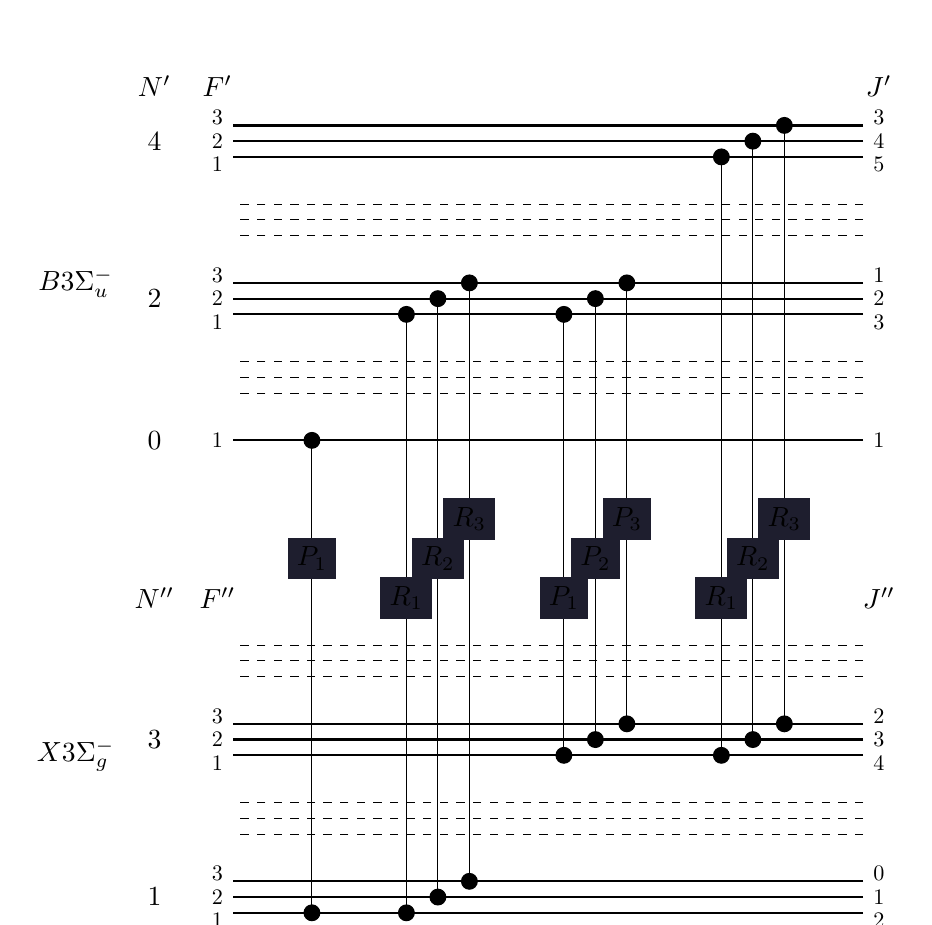
\begin{tikzpicture}
        \node at (-1,10.5) {$N'$};
        \node at (-0.2,10.5) {$F'$};
        \node at (8.2,10.5) {$J'$};

        \node at(-2,8) {$B\state{3}{\Sigma}_u^{-}$};

        \draw[thick] (8,10) -- (0,10);
        \node[scale=0.8] at (-0.2,10.1) {3};
        \node[scale=0.8] at (8.2,10.1) {3};
        \draw[thick] (8,9.8) -- (0,9.8);
        \node[scale=0.8] at (-0.2,9.8) {2};
        \node[scale=0.8] at (8.2,9.8) {4};
        \node at (-1,9.8) {4};
        \draw[thick] (8,9.6) -- (0,9.6);
        \node[scale=0.8] at (-0.2,9.5) {1};
        \node[scale=0.8] at (8.2,9.5) {5};

        \draw[dashed] (8,9) -- (0,9);
        \draw[dashed] (8,8.8) -- (0,8.8);
        \draw[dashed] (8,8.6) -- (0,8.6);

        \draw[thick] (8,8) -- (0,8);
        \node[scale=0.8] at (-0.2,8.1) {3};
        \node[scale=0.8] at (8.2,8.1) {1};
        \draw[thick] (8,7.8) -- (0,7.8);
        \node[scale=0.8] at (-0.2,7.8) {2};
        \node[scale=0.8] at (8.2,7.8) {2};
        \node at (-1,7.8) {2};
        \draw[thick] (8,7.6) -- (0,7.6);
        \node[scale=0.8] at (-0.2,7.5) {1};
        \node[scale=0.8] at (8.2,7.5) {3};

        \draw[dashed] (8,7) -- (0,7);
        \draw[dashed] (8,6.8) -- (0,6.8);
        \draw[dashed] (8,6.6) -- (0,6.6);

        \draw[thick] (8,6) -- (0,6);
        \node[scale=0.8] at (-0.2,6) {1};
        \node[scale=0.8] at (8.2,6) {1};
        \node at (-1,6) {0};

        \node at (-1,4) {$N''$};
        \node at (-0.2,4) {$F''$};
        \node at (8.2,4) {$J''$};

        \node at(-2,2) {$X\state{3}{\Sigma}_g^{-}$};

        \draw[dashed] (8,3.4) -- (0,3.4);
        \draw[dashed] (8,3.2) -- (0,3.2);
        \draw[dashed] (8,3) -- (0,3);

        \draw[thick] (8,2.4) -- (0,2.4);
        \node[scale=0.8] at (-0.2,2.5) {3};
        \node[scale=0.8] at (8.2,2.5) {2};
        \draw[thick] (8,2.2) -- (0,2.2);
        \node[scale=0.8] at (-0.2,2.2) {2};
        \node[scale=0.8] at (8.2,2.2) {3};
        \node at (-1,2.2) {3};
        \draw[thick] (8,2) -- (0,2);
        \node[scale=0.8] at (-0.2,1.9) {1};
        \node[scale=0.8] at (8.2,1.9) {4};

        \draw[dashed] (8,1.4) -- (0,1.4);
        \draw[dashed] (8,1.2) -- (0,1.2);
        \draw[dashed] (8,1) -- (0,1);

        \draw[thick] (8,0.4) -- (0,0.4);
        \node[scale=0.8] at (-0.2,0.5) {3};
        \node[scale=0.8] at (8.2,0.5) {0};
        \draw[thick] (8,0.2) -- (0,0.2);
        \node[scale=0.8] at (-0.2,0.2) {2};
        \node[scale=0.8] at (8.2,0.2) {1};
        \node at (-1,0.2) {1};
        \draw[thick] (8,0) -- (0,0);
        \node[scale=0.8] at (-0.2,-0.1) {1};
        \node[scale=0.8] at (8.2,-0.1) {2};

        \draw (1,6) -- (1,0);
        \filldraw (1,6) circle (0.1);
        \filldraw (1,0) circle (0.1);
        \node[fill=base] at (1,4.5) {$P_1$};

        \draw (2.2,7.6) -- (2.2,0);
        \filldraw (2.2,7.6) circle (0.1);
        \filldraw (2.2,0) circle (0.1);
        \node[fill=base] at (2.2,4) {$R_1$};
        \draw (2.6,7.8) -- (2.6,0.2);
        \filldraw (2.6,7.8) circle (0.1);
        \filldraw (2.6,0.2) circle (0.1);
        \node[fill=base] at (2.6,4.5) {$R_2$};
        \draw (3,8) -- (3,0.4);
        \filldraw (3,8) circle (0.1);
        \filldraw (3,0.4) circle (0.1);
        \node[fill=base] at (3,5) {$R_3$};

        \draw (4.2,7.6) -- (4.2,2);
        \filldraw (4.2,7.6) circle (0.1);
        \filldraw (4.2,2) circle (0.1);
        \node[fill=base] at (4.2,4) {$P_1$};
        \draw (4.6,7.8) -- (4.6,2.2);
        \filldraw (4.6,7.8) circle (0.1);
        \filldraw (4.6,2.2) circle (0.1);
        \node[fill=base] at (4.6,4.5) {$P_2$};
        \draw (5,8) -- (5,2.4);
        \filldraw (5,8) circle (0.1);
        \filldraw (5,2.4) circle (0.1);
        \node[fill=base] at (5,5) {$P_3$};

        \draw (6.2,9.6) -- (6.2,2);
        \filldraw (6.2,9.6) circle (0.1);
        \filldraw (6.2,2) circle (0.1);
        \node[fill=base] at (6.2,4) {$R_1$};
        \draw (6.6,9.8) -- (6.6,2.2);
        \filldraw (6.6,9.8) circle (0.1);
        \filldraw (6.6,2.2) circle (0.1);
        \node[fill=base] at (6.6,4.5) {$R_2$};
        \draw (7,10) -- (7,2.4);
        \filldraw (7,10) circle (0.1);
        \filldraw (7,2.4) circle (0.1);
        \node[fill=base] at (7,5) {$R_3$};
    \end{tikzpicture}
    \caption{Primary branch transitions between rotational levels of the Schumann--Runge system of molecular oxygen.}
\end{figure}

\begin{figure}[H]
    \centering
    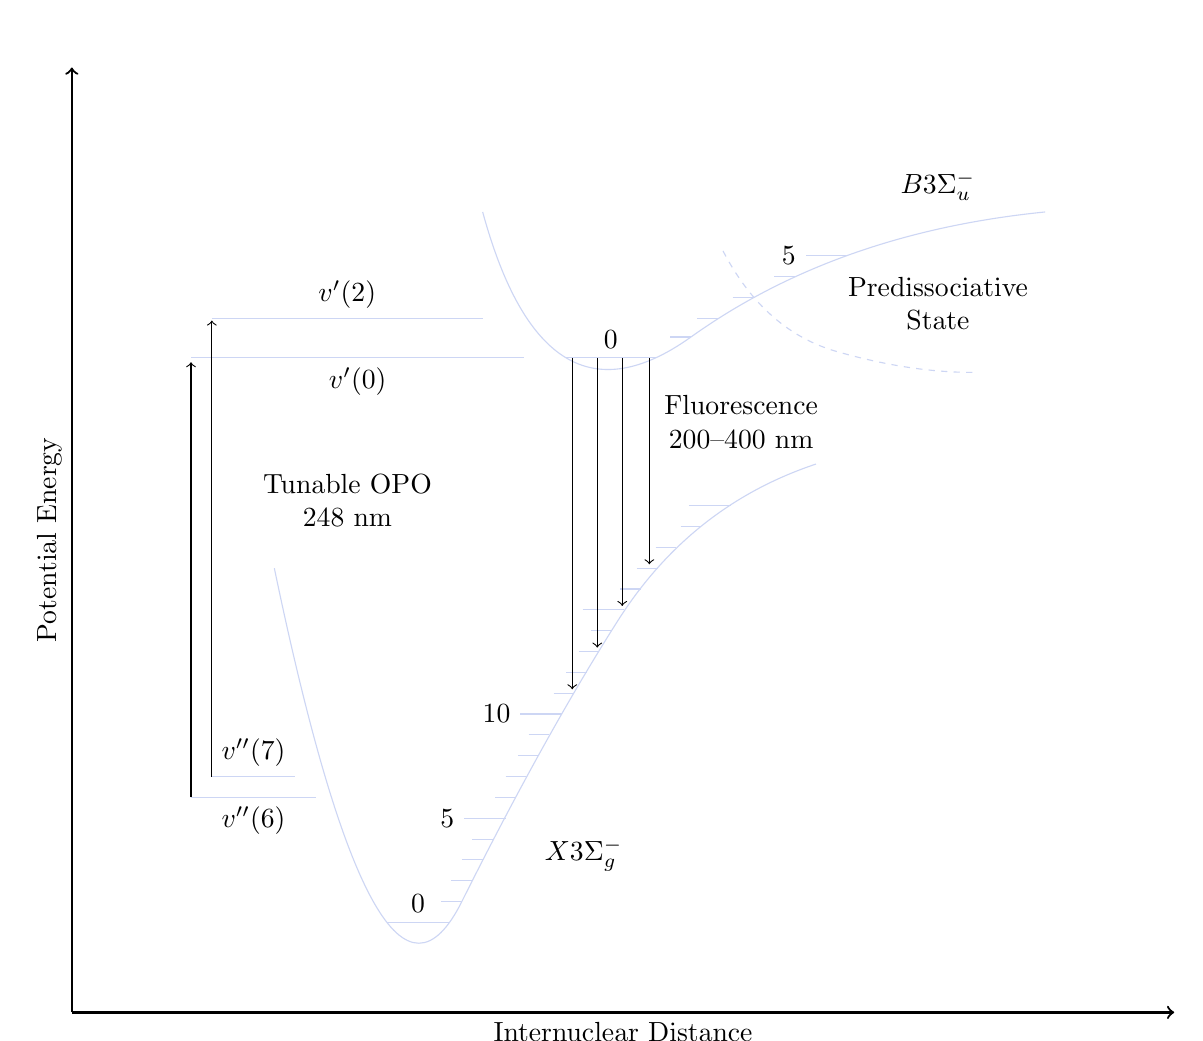
\begin{tikzpicture}
        % Excited state
        \path[draw=text] (6.2177, 11.1654) .. controls (6.7469, 9.2251) and (7.6288, 8.696) .. (8.8635, 9.5779) .. controls (10.0983, 10.4599) and (11.5976, 10.989) .. (13.3615, 11.1654);

        % Ground state
        \path[draw=text] (3.5719, 6.641) .. controls (4.4538, 2.4077) and (5.2476, 0.9966) .. (5.9531, 2.4077) .. controls (6.6587, 3.8188) and (7.3201, 5.0094) .. (7.9375, 5.9796) .. controls (8.5549, 6.9497) and (9.3927, 7.6112) .. (10.451, 7.964);

        % Predissociative state
        \path[draw=text,dash pattern=on 0.0794cm off 0.0794cm] (12.4354, 9.1281) .. controls (11.9063, 9.1281) and (11.333, 9.2163) .. (10.7156, 9.3927) .. controls (10.0983, 9.5691) and (9.6132, 10.0013) .. (9.2604, 10.6892);

        % Ground state energy levels
        \path[draw=text] (5.0006, 2.1431) -- (5.7944, 2.1431) node[midway,above] {$0$};
        \path[draw=text] (5.6885, 2.4077) -- (5.9531, 2.4077);
        \path[draw=text] (5.8208, 2.6723) -- (6.0854, 2.6723);
        \path[draw=text] (5.9531, 2.9369) -- (6.2177, 2.9369);
        \path[draw=text] (6.0854, 3.2015) -- (6.35, 3.2015);
        \path[draw=text] (6.5088, 3.466) -- (5.9796, 3.466) node[left] {$5$};
        \path[draw=text] (6.3765, 3.7306) -- (6.641, 3.7306);
        \path[draw=text] (6.5088, 3.9952) -- (6.7733, 3.9952);
        \path[draw=text] (6.6675, 4.2598) -- (6.9321, 4.2598);
        \path[draw=text] (6.7998, 4.5244) -- (7.0644, 4.5244);
        \path[draw=text] (7.2231, 4.789) -- (6.694, 4.789) node[left] {$10$};
        \path[draw=text] (7.1173, 5.0535) -- (7.3819, 5.0535);
        \path[draw=text] (7.276, 5.3181) -- (7.5406, 5.3181);
        \path[draw=text] (7.4348, 5.5827) -- (7.6994, 5.5827);
        \path[draw=text] (7.5935, 5.8473) -- (7.8581, 5.8473);
        \path[draw=text] (7.4877, 6.1119) -- (8.0169, 6.1119);
        \path[draw=text] (7.964, 6.3765) -- (8.2285, 6.3765);
        \path[draw=text] (8.1756, 6.641) -- (8.4402, 6.641);
        \path[draw=text] (8.4138, 6.9056) -- (8.6783, 6.9056);
        \path[draw=text] (8.7313, 7.1702) -- (8.9958, 7.1702);
        \path[draw=text] (8.8371, 7.4348) -- (9.3663, 7.4348);

        % Upper state energy levels
        \path[draw=text] (7.276, 9.3133) -- (8.4138, 9.3133) node[midway,above] {$0$};
        \path[draw=text] (8.599, 9.5779) -- (8.8635, 9.5779);
        \path[draw=text] (8.9429, 9.816) -- (9.2075, 9.816);
        \path[draw=text] (9.3927, 10.0806) -- (9.6573, 10.0806);
        \path[draw=text] (9.9219, 10.3452) -- (10.1865, 10.3452);
        \path[draw=text] (10.8479, 10.6098) -- (10.3188, 10.6098) node[left] {$5$};

        % Fluorescence lines
        \path[draw=text] (2.5135, 3.7306) -- (4.101, 3.7306) node[midway,below] {$v''(6)$};
        \path[draw=text] (2.7781, 3.9952) -- (3.8365, 3.9952) node[midway,above] {$v''(7)$};
        \path[draw=text] (2.5135, 9.3133) -- (6.7469, 9.3133) node[midway,below] {$v'(0)$};
        \path[draw=text] (2.7781, 9.816) -- (6.2177, 9.816) node[midway,above] {$v'(2)$};

        % Absorption arrows
        \draw[->] (2.5135, 3.7306) -- (2.5135, 9.2572);
        \draw[->] (2.7781, 3.9952) -- (2.7781, 9.7864);

        % Axes
        \draw[->,thick] (1, 1) -- (15, 1) node[midway,below] {Internuclear Distance};
        \draw[->,thick] (1, 1) -- (1, 13) node[midway,above,rotate=90] {Potential Energy};

        % Fluorescence arrows
        \draw[->] (7.3554, 9.3133) -- (7.3554, 5.1035);
        \draw[->] (7.6729, 9.3133) -- (7.6729, 5.6327);
        \draw[->] (7.9904, 9.3133) -- (7.9904, 6.1619);
        \draw[->] (8.3344, 9.3133) -- (8.3344, 6.691);

        % Labels
        \node at(7.5, 3) {$X\state{3}{\Sigma}_g^{-}$};
        \node at(12, 11.5) {$B\state{3}{\Sigma}_u^{-}$};
        \node[align=center] at(12, 10) {Predissociative\\State};
        \node[align=center] at(9.5, 8.5) {Fluorescence\\200--400 nm};
        \node[align=center] at(4.5, 7.5) {Tunable OPO\\248 nm};
    \end{tikzpicture}
    \caption{Potential energy diagram for the two electronic states of the Schumann--Runge band system.}
\end{figure}


\appendix

\chapter{Diatomic Constants}
\label{a:diatomic_constants}

\begin{table}[H]
    \centering
    \caption{Diatomic constants for \ce{^{16}O2} \cite{nistConstantsDiatomicMolecules2025}.}
    \label{t:diatomic_constants_for_o2}
    \begin{tabular}{cccc}
        \toprule
        Symbol            & \multicolumn{2}{c}{State}    & Units                                           \\
        \cmidrule(lr){2-3}
        & $X\state{3}{\Sigma}_g^{-}$ & $B\state{3}{\Sigma}_u^{-}$ &                  \\
        \midrule
        \multicolumn{4}{c}{\textit{Electronic}}                                                            \\
        \cmidrule(lr){1-4}
        $T_e$           & \num{0}                      & \num{49793.28}               & \unit{cm^{-1}}   \\
        \multicolumn{4}{c}{\textit{Vibrational}}                                                           \\
        \cmidrule(lr){1-4}
        $\omega_e$      & \num{1580.19(3)}             & \num{709.31}                 & \unit{cm^{-1}}   \\
        $\omega_ex_e$ & \num{11.98(1)}               & \num{10.65}                  & \unit{cm^{-1}}   \\
        $\omega_ey_e$ & \num{0.0474(7)}              & \num{-0.139}                 & \unit{cm^{-1}}   \\
        $\omega_ez_e$ & \num{-0.00127(3)}            &                              & \unit{cm^{-1}}   \\
        \multicolumn{4}{c}{\textit{Rotational}}                                                            \\
        \cmidrule(lr){1-4}
        $B_e$           & \num{1.4376766}              & \num{0.8190(2)}              & \unit{cm^{-1}}   \\
        $\alpha_e$      & \num{0.0159(3)}              & \num{0.01206}                & \unit{cm^{-1}}   \\
        $\gamma_e$      &                              & \num{-5.5(6)e-4}             & \unit{cm^{-1}}   \\
        $\delta_e$      &                              &                              & \unit{cm^{-1}}   \\
        \multicolumn{4}{c}{\textit{Centrifugal Distortion}}                                                \\
        \cmidrule(lr){1-4}
        $D_e$           &                              &                              & \unit{cm^{-1}}   \\
        $\beta_e$       &                              &                              & \unit{cm^{-1}}   \\
        \multicolumn{4}{c}{\textit{Spin-Splitting}}                                                        \\
        \cmidrule(lr){1-4}
        $\lambda$         &                              &                              & \unit{cm^{-1}}   \\
        $\gamma$          &                              &                              & \unit{cm^{-1}}   \\
        \multicolumn{4}{c}{\textit{Other}}                                                                 \\
        \cmidrule(lr){1-4}
        $H_e$           &                              &                              & \unit{cm^{-1}}   \\
        $r_e$           &                              &                              & \unit{\angstrom} \\
        $\nu_{00}$        &                              &                              & \unit{cm^{-1}}   \\
        \bottomrule
    \end{tabular}
\end{table}


\chapter{Notation for Diatomic Constants}
\label{a:notation_for_diatomic_constants}

\begin{table}[H]
    \centering
    \caption{Notation for diatomic constants \cite{herzbergMolecularSpectraMolecular1950,nistDiatomicSpectralDatabase2018a,nistDiatomicSpectralDatabase2018}.}
    \label{t:notation}
    \begin{tabular}{clc}
        \toprule
        Symbol            & Definition                                                                   & Units            \\
        \midrule
        \multicolumn{3}{c}{\textit{Electronic}}                                                                             \\
        \cmidrule(lr){1-3}
        $T_e$           & Minimum electronic energy                                                    & \unit{cm^{-1}}   \\
        \multicolumn{3}{c}{\textit{Vibrational}}                                                                            \\
        \cmidrule(lr){1-3}
        $G$               & Vibrational energy                                                           & \unit{cm^{-1}}   \\
        $\omega_e$      & Vibrational constant -- first term                                           & \unit{cm^{-1}}   \\
        $\omega_ex_e$ & Vibrational constant -- second term                                          & \unit{cm^{-1}}   \\
        $\omega_ey_e$ & Vibrational constant -- third term                                           & \unit{cm^{-1}}   \\
        $\omega_ez_e$ & Vibrational constant -- fourth term                                          & \unit{cm^{-1}}   \\
        \multicolumn{3}{c}{\textit{Rotational}}                                                                             \\
        \cmidrule(lr){1-3}
        $B_e$           & Rotational constant -- equilibrium                                           & \unit{cm^{-1}}   \\
        $\alpha_e$      & Rotational constant -- first term                                            & \unit{cm^{-1}}   \\
        $\gamma_e$      & Rotational constant -- second term (rotation-vibration interaction constant) & \unit{cm^{-1}}   \\
        $\delta_e$      & Rotational constant -- third term                                            & \unit{cm^{-1}}   \\
        \multicolumn{3}{c}{\textit{Centrifugal Distortion}}                                                                 \\
        \cmidrule(lr){1-3}
        $D_e$           & Centrifugal distortion constant -- equilibrium                               & \unit{cm^{-1}}   \\
        $\beta_e$       & Centrifugal distortion constant -- first term                                & \unit{cm^{-1}}   \\
        \multicolumn{3}{c}{\textit{Spin-Splitting}}                                                                         \\
        \cmidrule(lr){1-3}
        $\lambda$         & Spin-spin coupling parameter                                                 & \unit{cm^{-1}}   \\
        $\gamma$          & Spin-rotation coupling parameter                                             & \unit{cm^{-1}}   \\
        \multicolumn{3}{c}{\textit{Other}}                                                                                  \\
        \cmidrule(lr){1-3}
        $H_e$           & Sixth-order rotational constant                                              & \unit{cm^{-1}}   \\
        $r_e$           & Equilibrium internuclear distance                                            & \unit{\angstrom} \\
        $\nu_{00}$        & Position of $0\dash0$ band                                                   & \unit{cm^{-1}}   \\
        \bottomrule
    \end{tabular}
\end{table}


\printbibliography
\addcontentsline{toc}{chapter}{Bibliography}

\end{document}
